\documentclass{standalone}
\usepackage{tikz}
\usepackage{hyperref}

\usetikzlibrary{shadows,calc,math,shadings}


\newcommand{\html}[2]{\href{../html/#1/explanations.html}{#2}}



\begin{document}

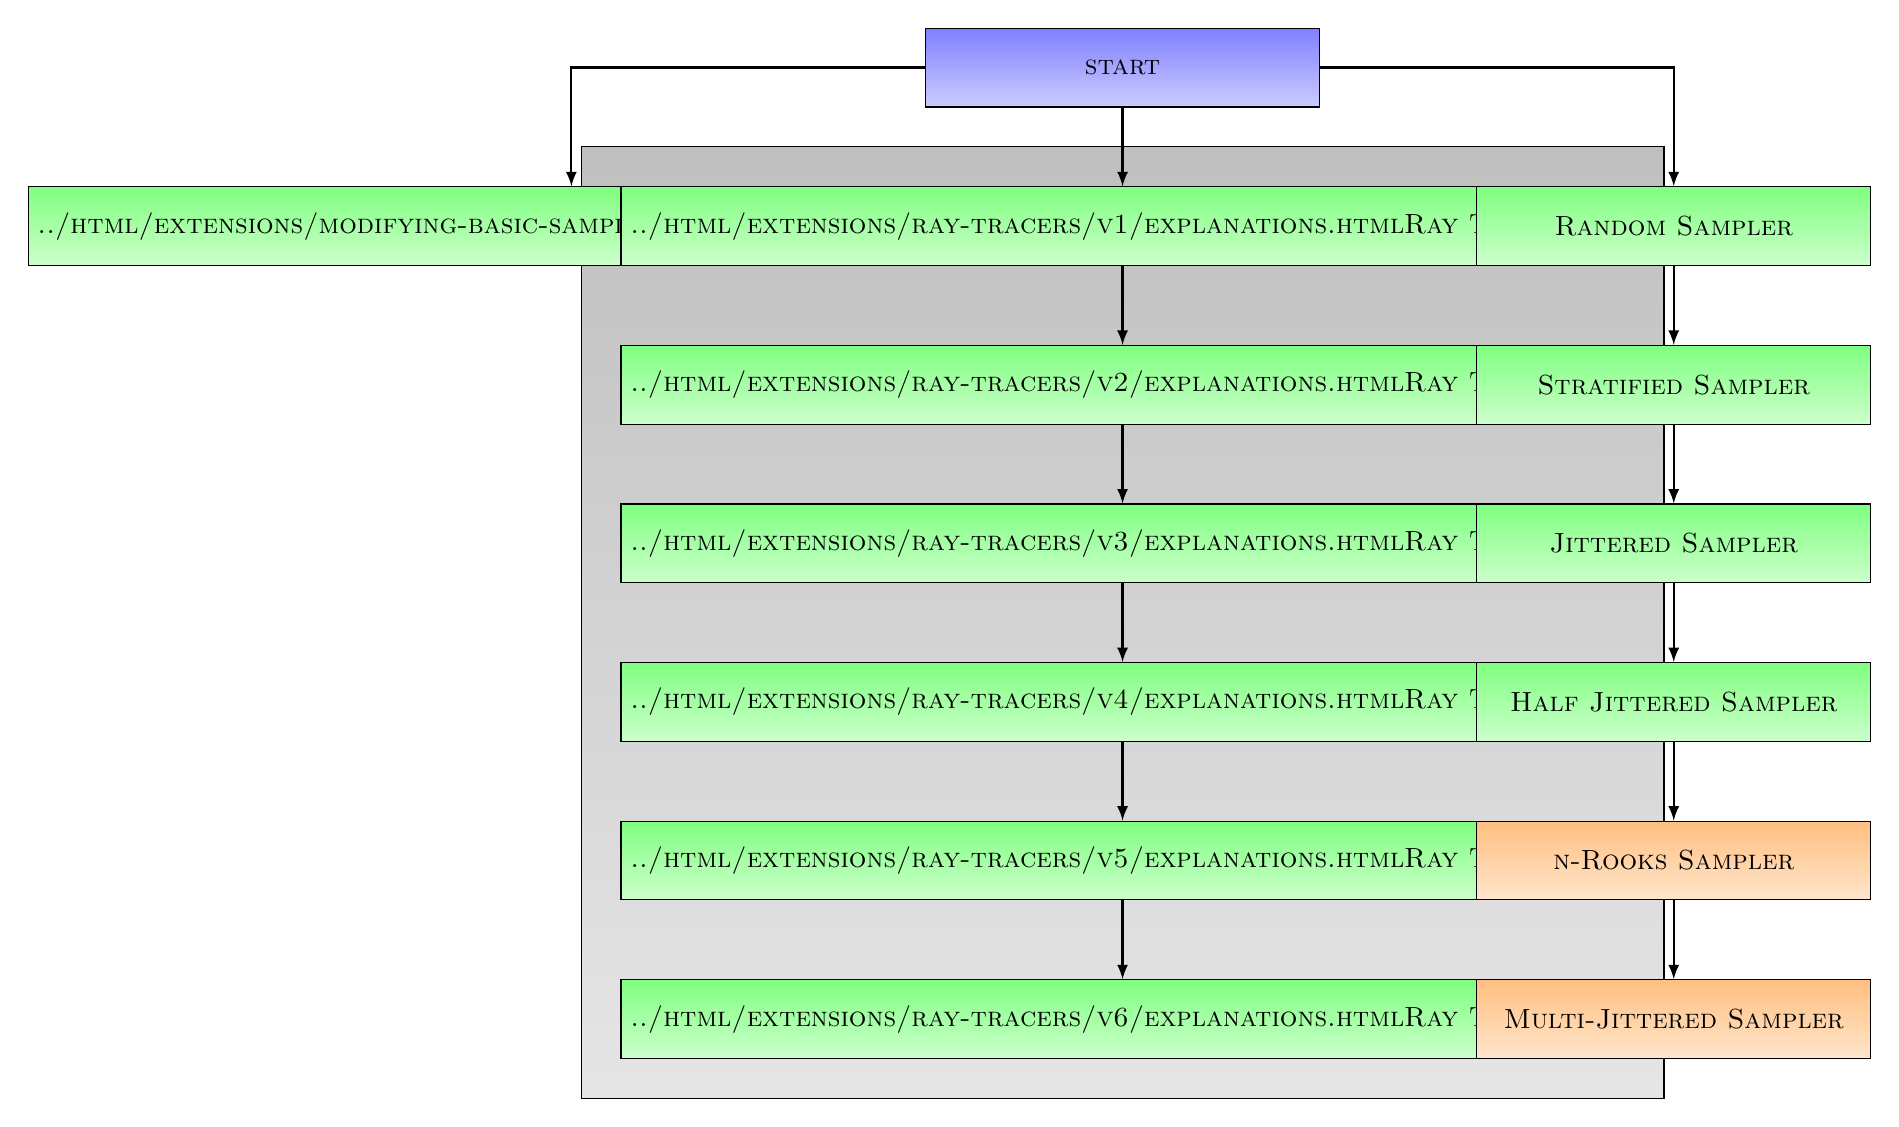
\begin{tikzpicture}[extension/.style={draw,minimum width=5cm,minimum height=1cm,font=\scshape},
                    dependency/.style={thick,latex-},
                    area/.style={top color=gray!50,bottom color=gray!20},
                    easy/.style={top color=green!50,bottom color=green!20},
                    medium/.style={top color=orange!50,bottom color=orange!20},
                    hard/.style={top color=red!50,bottom color=red!20}]
  \pgfdeclarelayer{background}
  \pgfsetlayers{background,main}

  \begin{pgfonlayer}{main}
    \node[extension,top color=blue!50,bottom color=blue!20] (start) {start};

    \node[extension,anchor=north,easy] (modifying-basic-sample) at ($ (start.south) + (-7,-1) $) {\html{extensions/modifying-basic-sample}{Basic Sample}};
    \draw[dependency] (modifying-basic-sample) |- (start);

    \node[extension,anchor=north,easy] (ray tracer v1) at ($ (start.south) + (0,-1) $) {\html{extensions/ray-tracers/v1}{Ray Tracer v1}};
    \draw[dependency] (ray tracer v1) -- (start);

    \node[extension,anchor=north,easy] (ray tracer v2) at ($ (ray tracer v1.south) + (0,-1) $) {\html{extensions/ray-tracers/v2}{Ray Tracer v2}};
    \draw[dependency] (ray tracer v2) -- (ray tracer v1);

    \node[extension,anchor=north,easy] (ray tracer v3) at ($ (ray tracer v2.south) + (0,-1) $) {\html{extensions/ray-tracers/v3}{Ray Tracer v3}};
    \draw[dependency] (ray tracer v3) -- (ray tracer v2);

    \node[extension,anchor=north,easy] (ray tracer v4) at ($ (ray tracer v3.south) + (0,-1) $) {\html{extensions/ray-tracers/v4}{Ray Tracer v4}};
    \draw[dependency] (ray tracer v4) -- (ray tracer v3);

    \node[extension,anchor=north,easy] (ray tracer v5) at ($ (ray tracer v4.south) + (0,-1) $) {\html{extensions/ray-tracers/v5}{Ray Tracer v5}};
    \draw[dependency] (ray tracer v5) -- (ray tracer v4);

    \node[extension,anchor=north,easy] (ray tracer v6) at ($ (ray tracer v5.south) + (0,-1) $) {\html{extensions/ray-tracers/v6}{Ray Tracer v6}};
    \draw[dependency] (ray tracer v6) -- (ray tracer v5);

    \node[extension,anchor=north,easy] (random sampler) at ($ (start.south) + (7,-1) $) {Random Sampler};
    \draw[dependency] (random sampler) |- (start);

    \node[extension,anchor=north,easy] (stratified sampler) at ($ (random sampler.south) + (0,-1) $) {Stratified Sampler};
    \draw[dependency] (stratified sampler) -- (random sampler);

    \node[extension,anchor=north,easy] (jittered sampler) at ($ (stratified sampler.south) + (0,-1) $) {Jittered Sampler};
    \draw[dependency] (jittered sampler) -- (stratified sampler);

    \node[extension,anchor=north,easy] (half jittered sampler) at ($ (jittered sampler.south) + (0,-1) $) {Half Jittered Sampler};
    \draw[dependency] (half jittered sampler) -- (jittered sampler);

    \node[extension,anchor=north,medium] (nrooks sampler) at ($ (half jittered sampler.south) + (0,-1) $) {n-Rooks Sampler};
    \draw[dependency] (nrooks sampler) -- (half jittered sampler);

    \node[extension,anchor=north,medium] (multijittered sampler) at ($ (nrooks sampler.south) + (0,-1) $) {Multi-Jittered Sampler};
    \draw[dependency] (multijittered sampler) -- (nrooks sampler);

  \end{pgfonlayer}

  \begin{pgfonlayer}{background}
    \draw[area] ($ (ray tracer v1.north west) + (-0.5,0.5) $) rectangle ($ (ray tracer v6.south east) + (0.5,-0.5) $);
  \end{pgfonlayer}
\end{tikzpicture}

\end{document}